\let\negmedspace\undefined
\let\negthickspace\undefined
\documentclass[journal]{IEEEtran}
\usepackage[a5paper, margin=10mm, onecolumn]{geometry}
%\usepackage{lmodern} % Ensure lmodern is loaded for pdflatex
\usepackage{tfrupee} % Include tfrupee package

\setlength{\headheight}{1cm} % Set the height of the header box
\setlength{\headsep}{0mm}     % Set the distance between the header box and the top of the text

\usepackage{gvv-book}
\usepackage{gvv}
\usepackage{cite}
\usepackage{amsmath,amssymb,amsfonts,amsthm}
\usepackage{algorithmic}
\usepackage{graphicx}
\usepackage{textcomp}
\usepackage{xcolor}
\usepackage{txfonts}
\usepackage{listings}
\usepackage{enumitem}
\usepackage{mathtools}
\usepackage{gensymb}
\usepackage{comment}
\usepackage[breaklinks=true]{hyperref}
\usepackage{tkz-euclide} 
\usepackage{listings}
% \usepackage{gvv}                                        
\def\inputGnumericTable{}                                 
\usepackage[latin1]{inputenc}                                
\usepackage{color}                                            
\usepackage{array}                                            
\usepackage{longtable}                                       
\usepackage{calc}                                             
\usepackage{multirow}                                         
\usepackage{hhline}                                           
\usepackage{ifthen}                                           
\usepackage{lscape}
\begin{document}

\bibliographystyle{IEEEtran}
\vspace{3cm}

\title{1.5.35}
\author{EE24BTECH11012 - Bhavanisankar G S}
% \maketitle
% \newpage
% \bigskip
{\let\newpage\relax\maketitle}

\renewcommand{\thefigure}{\theenumi}
\renewcommand{\thetable}{\theenumi}
\setlength{\intextsep}{10pt} % Space between text and floats


\numberwithin{equation}{enumi}
\numberwithin{figure}{enumi}
\renewcommand{\thetable}{\theenumi}

\textbf{QUESTION} \\
The mid-point of segment $\vec{AB}$ is the point $\vec{P}$ \vec{0,4} . If the coordinates of $\vec{B}$ are \vec{-2,3} then coordinates of $\vec{A}$ are \hfill \brak{10, 2011} \\
\textbf{SOLUTION} \\
\begin{table}[h!]    
  \centering
  \begin{table}[!ht]
	\centering
	\setlength{\extrarowheight}{8pt}
	\begin{tabular}{|c|c|c|}
    \hline
    \textbf{Variable name} & \textbf{Description} & \textbf{Formula}\\ 
    \hline
    A & The point in 2-D plane whose coordinates are to be found. &  $\vec{M} = \frac{\vec{A} + \vec{B}}{2}$\\
    \hline 
		B & The point in 2-D plane with coordinates \vec{-2,3} & $B$ = \brak{-2,3} \\
    \hline
		M & The midpoint of the line-segment \vec{AB} with coordinates \vec{0,4} & $M$ = \brak{0,4} $A$ = ? \\
    \hline   
    \end{tabular}
	\vspace{2mm}
	\caption{Variables Used}
	\label{table_1.5.35}
\end{table}

	\caption{Variables used}
  \label{tab.1.5.35}
\end{table}
\emph{Given} : \\
Coordinates of B = \vec{-2,3} \\
Coordinates of midpoint \brak{say M}  = \vec{0,4} \\
\emph{To Find} : \\
Coordinates of A. \\
We know that the mid-point of two points, which can be treated as vectors $\vec{A}$ and $\vec{B}$ is 
\begin{equation}
	\label{eq1}
	\begin{split}
	 \vec{M} &= \frac{\vec{A} + \vec{B}}{2} 
	\end{split}
\end{equation}
\begin{equation}
	\begin{split}
		\implies \vec{A} &= 2\vec{M} - \vec{B} \\
 &= 2\myvec{ 0 \\ 4 } - \myvec{-2 \\ 3 } \\
 &= \myvec{0 \\ 8} - \myvec{-2 \\ 3} \\
		&= \myvec{2 \\ 5} 
	\end{split}
\end{equation}

Hence, the coordinates of point $\vec{A}$ are \vec{2,5} .

\begin{figure}[h] % 'h' for here (positioning of the figure)
    \centering
    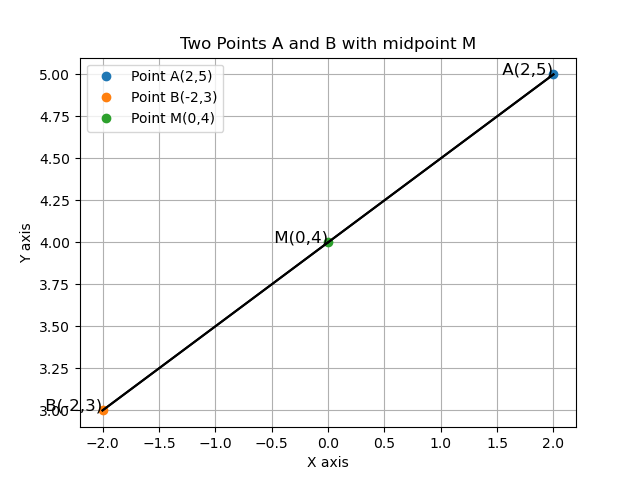
\includegraphics[width=0.8\textwidth]{figs/Graph1.png}
	\caption{A plot of the given question.}
    \label{fig:Plot1}
\end{figure}
 
\end{document}
